\section{Class Diagram Design}

\subsection{Class Identification}

The class diagram represents the static structure of the Decentralized Smart Power Grid System by identifying the primary classes, their attributes, operations, and relationships.
\clearpage
\subsection{Class Diagram}

\begin{figure}[H]
    \centering
    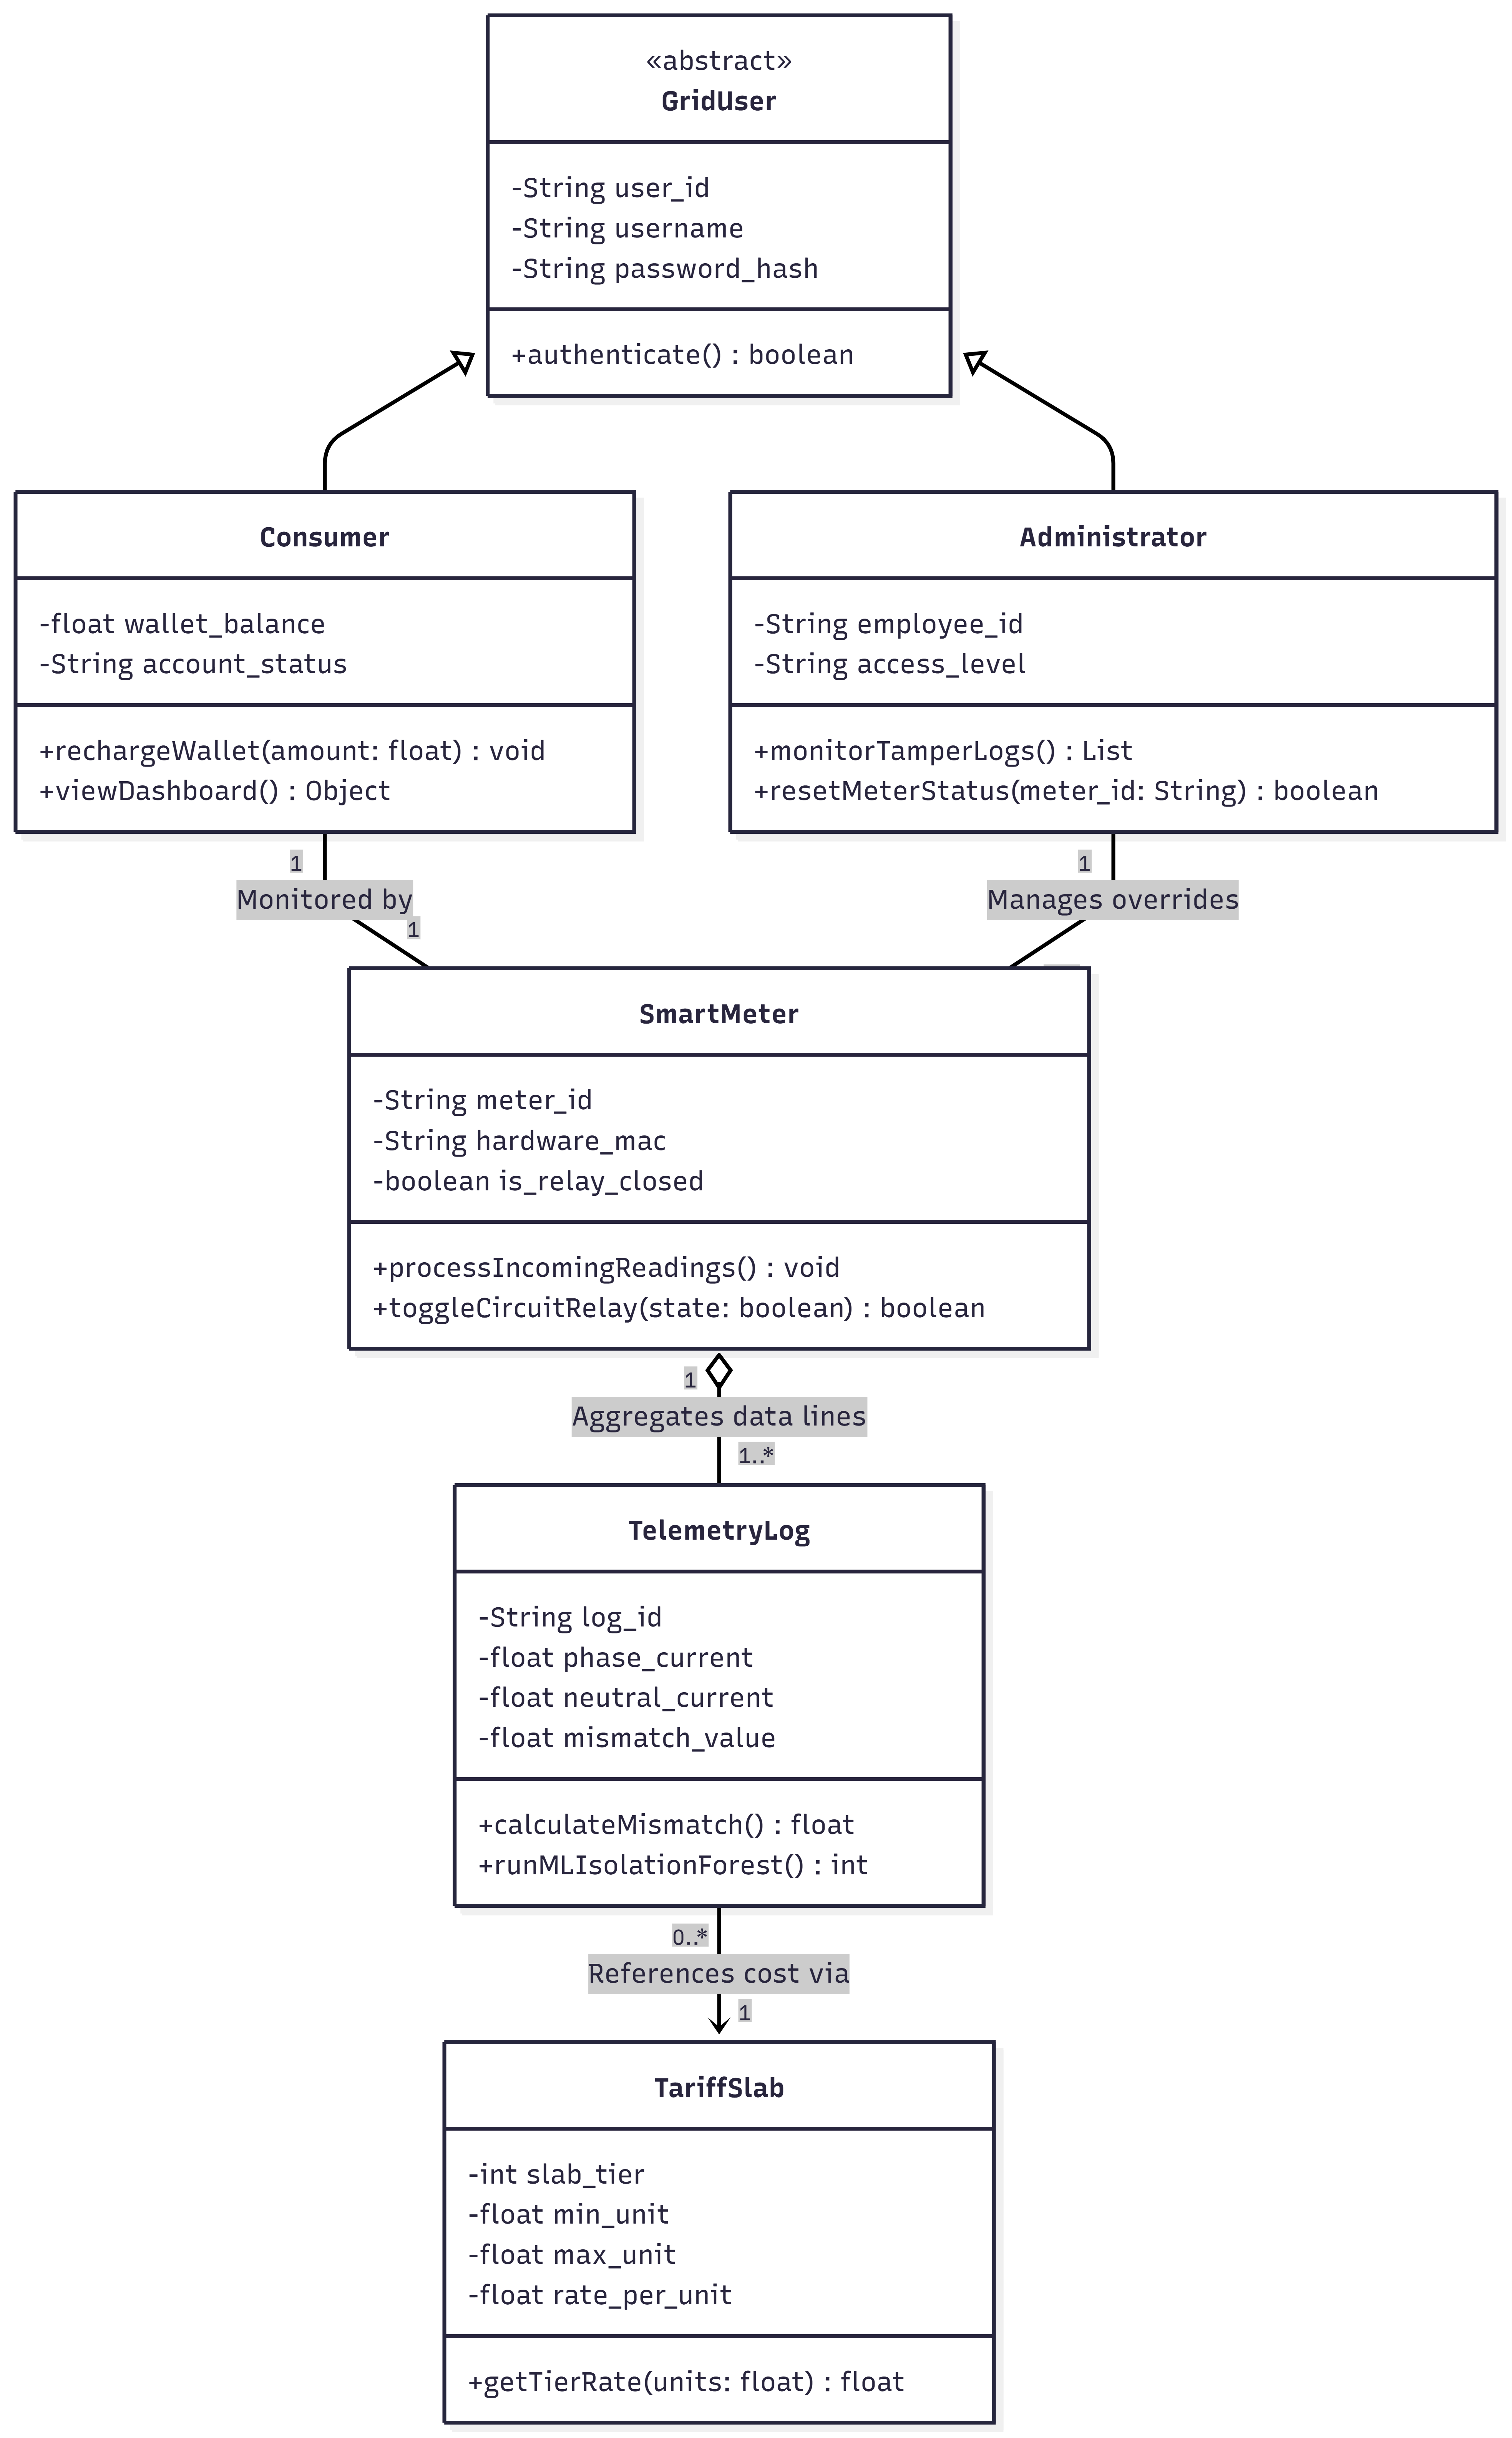
\includegraphics[
        width=\textwidth,
        height=0.81\textheight,
        keepaspectratio
    ]{graphics/class diagram.png}
    \caption{Class Diagram of the Decentralized Smart Power Grid System}
    \label{fig:class}
\end{figure}


\subsection{Class Description}

The principal classes include Consumer, Smart Meter, Backend Server, Smart Contract, Database, and Administrator. These classes collaborate to collect energy consumption data, process prepaid billing through blockchain technology, detect abnormal usage, and provide real-time monitoring facilities.